\itemhead{习题3.1 · 第16题（教材p.78）}{XJ-B1-C03-HW-P078-Y1352}
\label{XJ-B1-C03-HW-P078-Y1352}
{\footnotesize 湘教版教材p.78 / PDF第85页 / 习题3.1 / 第16题}
\field{原题}{设函数 $\operatorname{sign}(x)$ 的定义为 $\operatorname{sign}(x)=\begin{cases}0,&x\le0,\\1,&x>0.\end{cases}$
\subq{1}画出该函数的图象；
\subq{2}探索利用函数 $\operatorname{sign}(x)$ 把分段函数写成一个解析式的方法，并具体尝试用一个解析式来写出上面第 9 题中的函数。
\par\textit{引用定位：习题3.1第9题，教材p.77（西红柿价格与上市时间折线图），对应题库条目 XJ-B1-C03-HW-P077-Y1227。}}
\field{参考答案}{（1）$x\le0$ 时画水平线 $y=0$，$(0,0)$ 实心；$x>0$ 时画 $y=1$，$(0,1)$ 空心。（2）第9题可写为 $P(t)=3-t/100+(3t/100-6)\operatorname{sign}(t-200)$，$0\le t\le300$。此处必须使用题目定义的0、1阶跃函数，不能套用通常的正负号函数。}
\begin{center}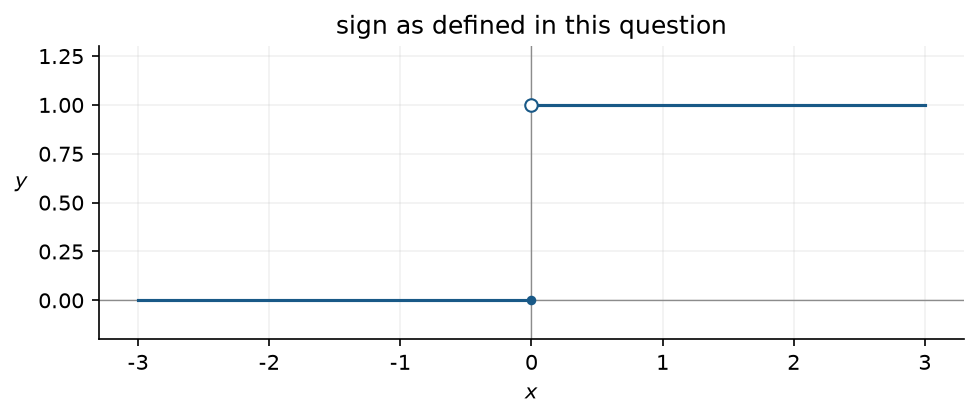
\includegraphics[width=.84\linewidth,height=.38\textheight,keepaspectratio]{figures/C03-HW078-16.png}\end{center}
\field{核对说明}{特殊定义提醒：本题sign为0/1阶跃函数，按其定义组织表达式；原题200处需检验，不能直接用常见的-1/0/1符号函数。}
{\small \field{关联知识}{F07 分段函数、绝对值及分段应用（教材帮p.86、91、92、93 / PDF95、100、101、102）}
\field{方法与易错点}{先列转折点和各段条件，再建立分段式，检查衔接、定义域与值域。 易错：跨段套公式；超额部分按全量收费；绝对值去号漏区间。}
\field{答案依据}{答案册相关题组：PDF第20、21、22页（册内页19、20、21）；按当前题库原题逐项重算，不按旧版题号机械对套。}}
